\chapter{Fundamentação Teórica}
\label{c.fundamentacaoteorica}

Em Ciência da Computação, compressão de dados é o processo de codificar as mesmas informações usando um número menor de bits, sem que haja distorção dos dados originais. Em se tratando de compressão de imagens, pode-se alcançar Esse processo é útil, pois reduz o consumo de recursos computacionais, como espaço em disco, ou utilização de banda de internet.

Considere as imagens abaixo.

\begin{figure}[h]
\caption{\small Codificador e Decodificado de Imagens}
\centering
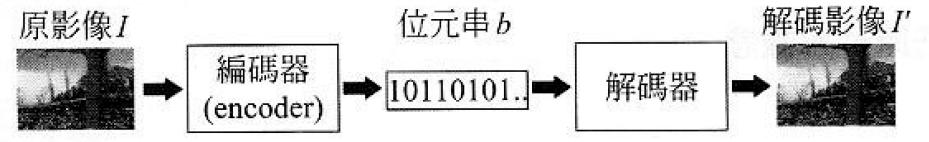
\includegraphics[scale=0.50]{figs/image_compression.jpg}
\label{f.imagecompressionbasics}
\legend{\small Fonte: Elaborada pelo autor.}
\end{figure}

Quando o sistema recebe a imagem original, ele manda para um codificador que converte a imagem original para um fluxo de bits. Um decodificador então recebe esse fluxo de bits e o transforma novamente na imagem. Caso o fluxo de bits final seja menor que o original, chamamos esse processo de Compressão de Imagem.

Durante a compressão de uma imagem, pode-se ter perda de dados durante o processo. Por essa razão, o decodificador não consegue reconstruir a imagem perfeitamente para seu estado inicial. Esse tipo de compressão é chamado de Lossy, e esse processo é irreversível. O processo no qual a imagem pode retornar ao seu estado inicial é chamado de {\em Lossless}, o qual é possível reduzir o tamanho em disco, sem ter perda de dados durante o processo, sendo esse um processo reversível.

\section{Métodos de Compressão de Imagem Sem Perda}
\label{s.lossless}

São os chamados tipos de compressão {\em Lossless}. Neles, como dito anteriormente, é possível restaurar todos os dados originais da Imagem ao descompacta-la. Esse tipo de compressão é geralmente usado para arquivos de imagem de extensão GIF, formato usado na internet o qual são permitidas animação de imagens e utilização de transparência.

De acordo com \citeauthoronline{losslessmethods} (\citeyear{losslessmethods}) define que compressão de imagens do tipo {\em Lossless}, também conhecidas como Compressão de Imagem Sem Perda, podem ser alcançadas através de Métodos de Codificação, Domínio Espacial, Domínio de Frequência, os quais são baseados em Transformadas, são uma combinação desses métodos.

Métodos de codificação são diretamente aplicados a imagens de formato RAW, o qual é o formato mais puro de uma imagem, normalmente sendo gerado a partir de câmeras profissionais. Esse formato acumula todos os dados necessários da imagem, como abertura da câmera, tipo da câmera, ISO utilizada, entre outras informações. O método de codificação trata a imagem como uma sequência de números discretos. Métodos comuns dessa incluem aritmética, Huffman, Lempel-Ziv Welch e Run-Length.

Métodos de domínio espacial são uma combinação de algoritmos de domínio espacial e métodos de codificação. Eles não somente operam diretamente nos tons de cinza, que são tons atribuidos a um pixel sendo 0 equivalente a branco e 100 equivalente a preto, como também tentam eliminar a redundância espacial. Essa redundância consiste na semelhança de pixels adjacentes de uma imagem. Um exemplo disso seria uma imagem de um avião passando no céu sem nuvens, na qual a informação relevante a ser transmitida é o avião, e o fundo é a parte da imagem azul cujo conteúdo da imagem é praticamente uniforme.

Na compressão de domínos de frequência, a imagem é representada usando uma base apropriada, com o objetivo de se obter um coeficiente de matriz pequeno. Transformada do Cosseno Discreto (DCT) e Transformada Wavelet são exemplos de compressão de domínio de frequência.

\subsection{Performance}
\label{ss.losslessperformance}

Perfomance em algoritmos do tipo {\em Lossless} pode ser especificados em termos de complexidade e eficiência.

A complexidade de um algoritmo de compressão de imagem é medida pelo número de operações aritméticas necessárias para realizar ambos processos de codificação e decodificação. Esse é um fator importante para aplicações que envolvem compressão online, onde a velocidade é crucial.

Eficiência de compressão é medida pela proporção de compressão ou pela taxa de bits. Proporção de compressão é o número de bits por pixel de uma imagem comprimida. Por exemplo, se uma imagem de dimensões 256x256 de 8 bits por pixel, é necessários 256 * 256 * 8 bits = 65.536 bytes quando armazenada em sua forma original. Se a imagem otimizada possuir 32.768 bytes, então a proporção de compressão será 65536 / 32768 = 2. Como a imagem possui dimensão de 256x256 = 65.536 pixels, o arquivo comprimido precisa de 32768 * 8 / 65536 = 4 bits, o qual será a taxa de bits necessária. A proporção de compressão portanto está associada a taxa de bits necessária. Sendo {\em CR} a proporção de compressão, {\em BR} a taxa de bits e {\em v} o número de bits por pixel de uma imagem não otimizada, temos a seguinte fórmula:

\[ CR = b / BR \]

\subsection{Métodos de Codificação}
\label{ss.codingmethod}

Nessa seção, serão abordados alguns algoritmos de codifição, bem como a explicação do método.

Para casos de codificação na qual uma imagem em duas dimensões será comprimida, existe a necessidade de convertê-la para uma sequência de uma dimensão. Para esse processo, chamamos de Linearização.

\subsubsection{Linearização}
\label{sss.linearlization}

A linearização não afeta a frequência da codificação, sendo esse método aplicado para alguns casos. Como Huffman depende somente da frequência dos diferentes tons de cinza, o método não é afetado pela linearização. Agora métodos como Liv-Zempel dependem da ordem dos tons de cinza, sendo então afetados por métodos de linearização.

Imagens possuem o que é chamado de redundância local.

\subsection{Métodos de Domínio Espacial}
\label{ss.spacialmethod}

\subsection{Métodos de Domínio de Frequência}
\label{ss.transformmethod}
%
% De acordo com \citeauthoronline{hackerdictionary} (\citeyear{hackerdictionary}) define um {\em hacker} como sendo uma pessoa que contenha as seguinte características:
%
% \begin{alineas}
%   \item Uma pessoa a qual aprecia aprender detalhes de uma linguagem de programação ou de um sistema;
%   \item Uma pessoa a qual aprecia programar ao invés de apenas teorizar;
%   \item Uma pessoa capaz de apreciar o {\em hackeamento} de outra pessoa;
%   \item Uma pessoa que aprende rapidamente uma linguagem de programação;
%   \item Uma pessoa que é perito em determinada linguagem de programação ou sistema computacional.
% \end{alineas}
